%File: formatting-instructions-latex-2024.tex
%release 2024.0
\documentclass[letterpaper]{article} % DO NOT CHANGE THIS
\usepackage{aaai24}  % DO NOT CHANGE THIS
\usepackage{times}  % DO NOT CHANGE THIS
\usepackage{helvet}  % DO NOT CHANGE THIS
\usepackage{courier}  % DO NOT CHANGE THIS
\usepackage[hyphens]{url}  % DO NOT CHANGE THIS
\usepackage{graphicx} % DO NOT CHANGE THIS
\urlstyle{rm} % DO NOT CHANGE THIS
\def\UrlFont{\rm}  % DO NOT CHANGE THIS
\usepackage{natbib}  % DO NOT CHANGE THIS AND DO NOT ADD ANY OPTIONS TO IT
\usepackage{caption} % DO NOT CHANGE THIS AND DO NOT ADD ANY OPTIONS TO IT
\frenchspacing  % DO NOT CHANGE THIS
\setlength{\pdfpagewidth}{8.5in}  % DO NOT CHANGE THIS
\setlength{\pdfpageheight}{11in}  % DO NOT CHANGE THIS
%
% These are recommended to typeset algorithms but not required. See the subsubsection on algorithms. Remove them if you don't have algorithms in your paper.
\usepackage{algorithm}
\usepackage{algorithmic}

%
% These are are recommended to typeset listings but not required. See the subsubsection on listing. Remove this block if you don't have listings in your paper.
\usepackage{newfloat}
\usepackage{listings}
\DeclareCaptionStyle{ruled}{labelfont=normalfont,labelsep=colon,strut=off} % DO NOT CHANGE THIS
\lstset{%
	basicstyle={\footnotesize\ttfamily},% footnotesize acceptable for monospace
	numbers=left,numberstyle=\footnotesize,xleftmargin=2em,% show line numbers, remove this entire line if you don't want the numbers.
	aboveskip=0pt,belowskip=0pt,%
	showstringspaces=false,tabsize=2,breaklines=true}
\floatstyle{ruled}
\newfloat{listing}{tb}{lst}{}
\floatname{listing}{Listing}
%
% Keep the \pdfinfo as shown here. There's no need
% for you to add the /Title and /Author tags.
\pdfinfo{
/TemplateVersion (2024.1)
}


\usepackage{makecell}

% DISALLOWED PACKAGES
% \usepackage{authblk} -- This package is specifically forbidden
% \usepackage{balance} -- This package is specifically forbidden
% \usepackage{color (if used in text)
% \usepackage{CJK} -- This package is specifically forbidden
% \usepackage{float} -- This package is specifically forbidden
% \usepackage{flushend} -- This package is specifically forbidden
% \usepackage{fontenc} -- This package is specifically forbidden
% \usepackage{fullpage} -- This package is specifically forbidden
% \usepackage{geometry} -- This package is specifically forbidden
% \usepackage{grffile} -- This package is specifically forbidden
% \usepackage{hyperref} -- This package is specifically forbidden
% \usepackage{navigator} -- This package is specifically forbidden
% (or any other package that embeds links such as navigator or hyperref)
% \indentfirst} -- This package is specifically forbidden
% \layout} -- This package is specifically forbidden
% \multicol} -- This package is specifically forbidden
% \nameref} -- This package is specifically forbidden
% \usepackage{savetrees} -- This package is specifically forbidden
% \usepackage{setspace} -- This package is specifically forbidden
% \usepackage{stfloats} -- This package is specifically forbidden
% \usepackage{tabu} -- This package is specifically forbidden
% \usepackage{titlesec} -- This package is specifically forbidden
% \usepackage{tocbibind} -- This package is specifically forbidden
% \usepackage{ulem} -- This package is specifically forbidden
% \usepackage{wrapfig} -- This package is specifically forbidden
% DISALLOWED COMMANDS
\nocopyright % -- Your paper will not be published if you use this command
% \addtolength -- This command may not be used
% \balance -- This command may not be used
% \baselinestretch -- Your paper will not be published if you use this command
% \clearpage -- No page breaks of any kind may be used for the final version of your paper
% \columnsep -- This command may not be used
% \newpage -- No page breaks of any kind may be used for the final version of your paper
% \pagebreak -- No page breaks of any kind may be used for the final version of your paperr
% \pagestyle -- This command may not be used
% \tiny -- This is not an acceptable font size.
% \vspace{- -- No negative value may be used in proximity of a caption, figure, table, section, subsection, subsubsection, or reference
% \vskip{- -- No negative value may be used to alter spacing above or below a caption, figure, table, section, subsection, subsubsection, or reference

\setcounter{secnumdepth}{0} %May be changed to 1 or 2 if section numbers are desired.

% The file aaai24.sty is the style file for AAAI Press
% proceedings, working notes, and technical reports.
%

% Title

% Your title must be in mixed case, not sentence case.
% That means all verbs (including short verbs like be, is, using,and go),
% nouns, adverbs, adjectives should be capitalized, including both words in hyphenated terms, while
% articles, conjunctions, and prepositions are lower case unless they
% directly follow a colon or long dash
\title{Image Classification with Mini-ResNet}
\author {
    % Authors
    Mike Chaberski
    and
    Mukesh Ethiraj
    and
    Dinesh Sathunuri
}
\affiliations {
    % Affiliations
    NYU Tandon School of Engineering\\
    mac937@nyu.edu, me2638@nyu.edu, ds7675@nyu.edu@nyu.edu
}

\begin{document}

\maketitle

\begin{abstract}
    A model with ResNet architecture and less than 5 million trainable parameters is herein designed for the task of
    image classification.
    The model is trained and evaluated on the CIFAR-10 dataset, which contains very small images across ten classes.
    Model definition, training, and evaluation code is available at https://github.com/mike10004/csgy6953-mp1.
\end{abstract}

\section{Overview}

Image classification, in the context of this machine learning effort, is the task of identifying the content of an image.
Models with a residual network (ResNet) architecture, that is, deep convolutional neural networks containing layers with
skip connections, have shown strong performance in the image classification task.
The original ResNet paper reported 93.5\% accuracy for a model trained and evaluated on the CIFAR-10 dataset~\cite{dblp:2015}.
Example CIFAR images are shown in Figure~\ref{fig1}.

\begin{figure}[b]
\centering
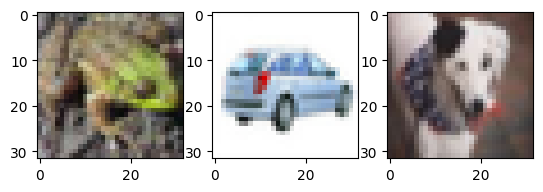
\includegraphics[width=0.95\columnwidth]{cifar-example-images}
\caption{CIFAR images from the frog, car, and dog classes.\cite{kriz:2009}}
\label{fig1}
\end{figure}

That original research studied models with large numbers of trainable parameters (though the ResNet architecture in
general requires many fewer parameters than standard CNN models to achieve good performance).
The smallest network in the original ResNet paper, ResNet-18, has 11.7 million parameters, according to
analysis of the PyTorch ResNet implementation by the Python package \textit{torch-summary}.

Documented herein is an effort to design and train a model with ResNet architecture that has under five
million parameters, with the objective of high accuracy on CIFAR-10.
Using model definition and training code adapted from a reference implementation~\cite{kl:2021}, model
hyperparameters and training strategies were determined through experimentation on a validation set.
The final model produced from this process achieves accuracy of 92.1\% on the CIFAR-10 test dataset.

\section{Methodology}

To design the optimal model for the classification task, a series of experiments was performed to
determine the best architecture, training strategies, and hyperparameters.
The types of training strategies considered included learning rate scheduling
and various regularization techniques.
For all experiments, the 50k-image CIFAR-10 training dataset was split into 90\% for training and 10\% for validation.
Alternatives were evaluated based on quantitative metrics such as validation accuracy as well as qualitative assessment
of loss curve trends.

\subsection{Architecture}

\begin{figure*}[t]
\centering
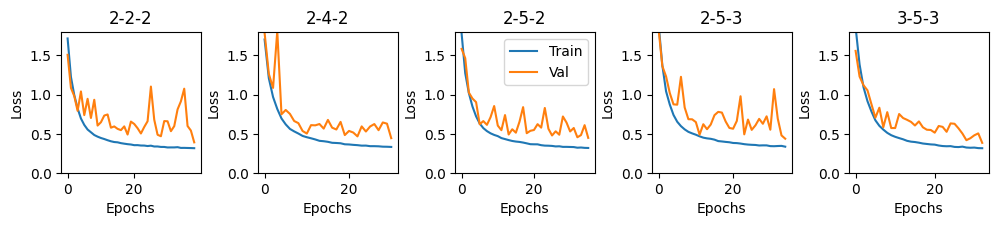
\includegraphics[width=0.99\textwidth]{loss-curves-5}
\caption{Training and validation loss by architecture with constant learning rate}
\label{fig2}
\end{figure*}

Our model definition code implements the core ResNet feature of convolutional layers with skip connections as a
pipeline of block sequences, where a block contains two convolutional layers, each with batch normalization, plus the
skip connection.
The number of block sequences in the pipeline and the lengths of the individual block sequences form a descriptor of a
given model architecture.
For example, the ResNet-18 model has four block sequences, each of length 2, and can be identified by the architecture
descriptor 2-2-2-2.

The original ResNet research exclusively defines pipelines with sequences of at least two blocks.
Architectures with four such block sequences have more than 5 million trainable parameters, thus candidate
architectures for our constraints must contain at most three sequences.
Based on these constraints, the following architectures are candidates for evaluation:
2-2-2, 2-4-2, 2-5-2, 2-5-3, and 3-5-3.
Because the upstream codebase explicitly defined a pipeline of four block sequences, it was adapted to support an
arbitrary number of block sequences.

For these initial experiments, hyperparameters and other training details are drawn from the original ResNet paper and
the upstream repository defaults.
The learning rate is set to $ 0.1 $ and models are trained for 40 epochs with
Stochastic Gradient Descent (SGD) at a batch size of 128.
Early experimentation showed that at higher epochs, validation accuracy would often
stagnate while training accuracy continued to improve.
To avoid the overfitting that comes with such a divergence, a policy was imposed where
training was stopped early if training accuracy reached between 97.5\% and 99.5\%,
depending on the experiment.

\begin{table}[b]
\centering
%\resizebox{.95\columnwidth}{!}{
\begin{tabular}{|l|r|}
    \firsthline
    Arch & Val Acc \%    \\
    \hline
    2-2-2 & 86.6    \\
    2-4-2 & 84.7    \\
    2-5-2 & 85.0    \\
    2-5-3 & 85.3    \\
    3-5-3 & 87.0    \\
    \lasthline
\end{tabular}
%}
\caption{Validation accuracy by architecture with constant learning rate}
\label{table1}
\end{table}

The results of the initial architecure experiment are shown in Table~\ref{table1}, and
the training and validation loss curves are shown in Figure~\ref{fig2}.
The most stable validation loss behavior was observed in architectures 2-4-2 and 3-5-3, but 2-2-2 and 3-5-3
have the greatest validation accuracy.
Before selecting a single architecture, we will consider learning rate scheduling to compare performance
of models that show more stable loss trends.

\subsection{Training Strategies}

\subsubsection{Learning Rate Scheduling}

The initial architecture experiments were conducted with a constant learning rate of 0.1.
Other approaches under consideration include: step scheduling, as used by the original ResNet paper;
cosine annealing, as implemented in the upstream codebase;
and adaptive scheduling that reduces the learning rate when validation loss plateaus.
For these experiments, training is stopped early if the training accuracy reaches 97.5\%.

\begin{table}[b]
\centering
%\resizebox{.95\columnwidth}{!}{
\begin{tabular}{|l|r|}
    \firsthline
    Arch/LRS & Val Acc \%    \\
    \hline
    2-2-2 Step & 86.7    \\
    3-5-3 Step & 87.3    \\
    2-2-2 Cosine annealing & 92.1    \\
    3-5-3 Cosine annealing & 92.0    \\
    2-2-2 Adaptive-plateau & 92.2    \\
    3-5-3 Adaptive-plateau & 91.7    \\
    \lasthline
\end{tabular}
%}
\caption{Validation accuracy by architecture and Learning Rate Scheduler}
\label{table2}
\end{table}

\begin{table}[b]
\centering
%\resizebox{.95\columnwidth}{!}{
\begin{tabular}{|r|r|r|}
    \firsthline
    \makecell{Input Layer \\ Dropout \% }  & \makecell{Hidden Layer \\ Dropout \% } & Val Acc \%    \\
    \hline
    0 & 0 & 91.8    \\
    20 & 0 & 91.4    \\
    20 & 20 & 91.2    \\
    20 & 50 & 89.7    \\
    \lasthline
\end{tabular}
%}
\caption{Validation accuracy under varying dropout rates. The input layer and hidden layer dropout rates are varied between 0 and 50\%.}
\label{table3}
\end{table}


\begin{figure*}[t]
\centering
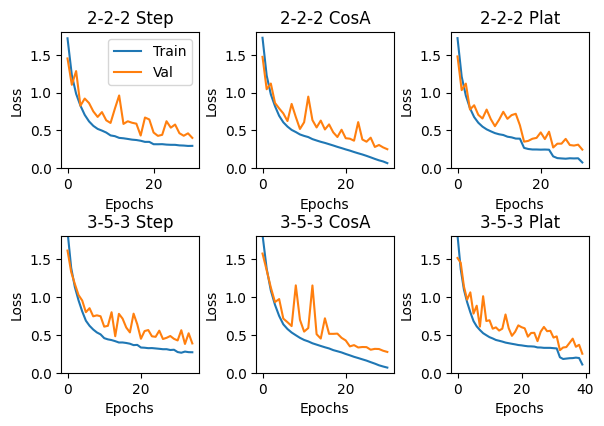
\includegraphics[width=0.8\textwidth]{experiment-lrschedule-2x3}
\caption{Training and validation loss by architecture and learning rate scheduler.}
\label{fig3}
\end{figure*}

\begin{figure}[t]
\centering
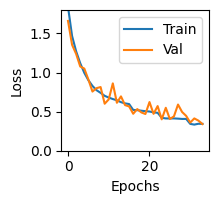
\includegraphics[width=0.55\columnwidth]{experiment-heavy-aug}
\caption{Training and validation loss under heavy augmentation}
\label{fig4}
\end{figure}

\begin{figure}[t]
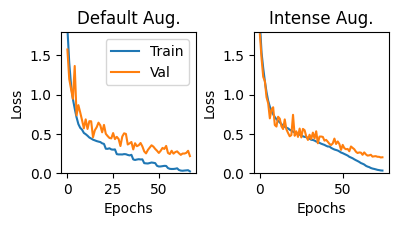
\includegraphics[width=0.98\columnwidth]{experiment-80epoch-augtypes}
\caption{Training and validation loss over 80 epochs with different augmentation and learning rate schedulers.}
\label{fig5}
\end{figure}


The results of the learning rate scheduler experiment, shown in Table~\ref{table2} and Figure~\ref{fig3}, indicate that
the cosine annealing and adaptive-plateau schedulers outperform the step scheduler under the current
parameterization.
The cosine annealing scheduler shows a strong downward trend in training loss while validation loss
stays stagnant.
This suggests that the cosine annealing scheduler is prone to overfitting, so the
adaptive-plateau scheduler will be selected by default for subsequent experiments.

The validation accuracy of the 2-2-2 and 3-5-3 architectures is about the same,
and we elect to use the 3-5-3 architecture, which has 4.9 million parameters, for its expressiveness
advantage, keeping in mind that the increased expressiveness means we must be vigilant
with respect to overfit.

\subsubsection{Regularization}

A suboptimal trend observed in the experiments above is the training loss continuing to decrease in later
epochs while the validation accuracy stagnates.
A possible explanation of this divergence is that the gradient reaches a local minimum, and further training
refines the model within that local neighborhood, resulting in improvements that do not generalize.
Subsequent minor increases in validation accuracy at that point are likely the result of random fluctuations as the
model becomes overfitted to the training data.

To reduce overfitting, several strategies for regularization were considered:
introducing dropout into training, increasing weight decay, and varying training data by augmentation.

\textit{Dropout.}
To test the effect of dropout, multiple dropout ``layers'' are inserted into the model at the input layer,
before and after the block sequence pipeline, and between each sequence in the block sequence pipeline.
Three dropout configurations were evaluated and compared to a zero-dropout configuration.
Among the dropout configurations, the input layer dropout rate was set at 20\%, while the hidden layer
dropout layers were assigned rates of 0\%, 20\%, and 50\% (the latter being recommended by \cite{JMLR:v15:srivastava14a}).
Models with dropout were trained up to 80 epochs, instead of the 40 epoch limit in above experiments,
to account for how dropout may delay convergence.
Early stopping was imposed at training accuracy of 97.5\%.

The validation accuracies under varying dropout configurations, displayed in Table~\ref{table3},
are not substantially different, and the configuration with no dropout achieves maximum validation accuracy.
The configuration in which the input layer dropout rate is 20\% but hidden layers have no dropout
is a close second, and it is worthy of consideration because the model may have learned a more robust
representation of the input, but there is not enough evidence to deviate from the default zero-dropout
configuration.

\textit{Weight Decay.}
Experiments varying weight decay from the default did not yield any useful insights.
A model trained with the default weight decay from the upstream repository, $0.0005 $,
was compared to models with weight decay values of $ 0.0 $, $ 0.00275 $, and $ 0.005 $.
The model trained with default weight decay achieved 92.3\% validation accuracy.
The model with zero decay performed slightly worse than the default, at 90.7\% accuracy, and
models with greater weight decay achieved about 80\% accuracy, with highly volatile validation
loss.
This does not rule out more granular investigation of weight decay parameter values, but does not
motivate us to pursue an alternative to the upstream default.

\textit{Data Augmentation.}
Unlike the experiments on dropout and weight decay, investigation into regularization by
intensifying data augmentation did show initial promise.
The default configuration, in which training data is augmented by random crop and random horizontal flip,
was compared to configurations with no augmentation and with heavier augmentation,
adding random rotation of up to 30 degrees in either direction.
As could be expected, the model trained with no augmentation performed worst,
achieving 88.1\% validation accuracy, compared to 90.4\% accuracy for the default configuration.
The loss curves for the configuration with no augmentation and default augmentation
are similar to those seen before, but the loss curves of the heavy augmentation
configuration, shown in Figure~\ref{fig4}, have an interesting feature.
Though that model achieves only 88.0\% accuracy, its
validation loss curve tracks its training loss curve very closely, suggesting that
the heavy augmentation makes the model less prone to overfitting.

This points to a potential avenue for improvement: use the cosine annealing learning rate scheduler,
which had previously been rejected for being prone to overfitting, paired with heavy
data augmentation, which mitigates overfitting.
To explore this potential, two models were trained out to 80 epochs, a baseline model with the
default augmentation and the adaptive plateau scheduler adopted above, and another with
heavy augmentation and a cosine annealing scheduler.

The heavy augmentation model achieves validation accuracy of 94.4\%, while the default
augmentation model achieves 94.2\%.
However, as Figure~\ref{fig5} shows, the training and validation loss curves eventually
diverge under both default and heavy augmentation.
The divergence only shows up in the heavy augmentation model after 40 epochs.

That divergence and the similar validation accuracy scores suggest that the heavy augmentation
method does not prevent overfitting.
The close tracking of training and validation loss was likely due to the heavy
augmentation inducing greater training loss,
while the same gradient characteristics were present as with default augmentation, so the models learned
in the same way.

\subsection{Hyperparameters}

Kernel sizes of 3, 5, and 7 for the convolution kernels within blocks were comparatively evaluated to establish the impact of the
block kernel size hyperparameter.
The impact of other hyperparameters, such as initial convolution kernel size,
the number of channels within blocks, and the pool size in the average pool
layer, are potentially worthy of consideration, but their values were fixed at the upstream defaults to reduce the
search space for this investigation.

The default kernel size is 3 in the upstream codebase, and the model trained with this kernel size achieved the
greatest valiation accuracy, at 89.4\%, while models trained with kernel sizes 5 achieved accuracies
of 88.8\% and 89.4\% respectively.
The training and validation loss curves are similar for all kernel sizes, with the training and validation
loss diverging slightly more at later epochs for kernel sizes 5 and 7.
The effect of varying the kernel size is not large, which is counterintuitive, considering the
the small dimensions of the CIFAR images.

\section{Results}

The analysis above suggests that a suitable choice of architecture, training strategy, and hyperparameters
is the following:

\begin{itemize}
    \item 3-5-3 architecture
    \item adaptive-plateau learning rate scheduler
    \item no dropout
    \item weight decay $ 0.0005 $
    \item random crop and random flip data augmentation
    \item convolution kernel size $ 3 $
\end{itemize}

A model with these characteristics model was trained with epoch limit of 80, and
training was stopped early when the training accuracy reached 97.5\% at epoch 56.
Validation accuracy was measured at each epoch, and the model with weights corresponding to the best
validation accuracy (92.8\%) was selected to be evaluated on the test data.

On the CIFAR-10 test dataset, which contains 10k images, the model's accuracy is 92.1\%,
comparable to the best validation accuracy.

Most avenues of investigation ended with the choice to use parameters specified by the original ResNet researchers or
the upstream codebase, or to use near equivalents.
This suggests either that those authors had performed adequate tuning already or that further exploration of variables,
with more granular and systematic examination, is warranted.
Grid search with cross validation would be an appropriate technique for such exploration, given sufficient time and
computing resources.

\bibliography{aaai24}

\end{document}
